\documentclass[12pt]{article}

\usepackage{hyperref}

% useful for formatting (align*, etc.) and for certain symbols (the QED box, etc.)
\usepackage{amsmath, amssymb, amsthm}

% for including graphics
\usepackage{graphicx}

% for conveniently specifying the spacing (\singlespacing, \doublespacing,
%    \onehalfspacing, etc.)
\usepackage{setspace}
\onehalfspacing

% this does some sort of symbol stuff
\usepackage{textcomp}

% A package for conveniently adjusting headers and such
\usepackage{fancyhdr}
\renewcommand{\headrulewidth}{0 pt}
\rhead{\textit{\thepage}}
\cfoot{}



% Set the margins
\usepackage[top=1.8cm, bottom=1.8cm, left=1.8cm, right=1.8cm]{geometry}

% Differently spaced itemize
\newenvironment{itemize*}%
  {\begin{itemize}%
  	\setlength{\parsep}{0pt}
    \setlength{\itemsep}{0pt}%
    \setlength{\parskip}{0pt}}%
  {\end{itemize}}
\newenvironment{enumerate*}%
  {\begin{enumerate}%
  	\setlength{\parsep}{0pt}
    \setlength{\itemsep}{0pt}%
    \setlength{\parskip}{0pt}}%
  {\end{enumerate}}


% set up a new command to insert a little bit of vertical space
% (use this BEFORE a line break)
\newcommand{\padding}{\vspace*{.5cm}}

% set up an environment to format each hw problem in
\newenvironment{problem}[1]{\noindent\textbf{#1.}}{\vspace*{.5cm}}

\newenvironment{proof*}{\par\noindent{\bf Proof}\quad}
               {\quad\vrule height 8pt depth 0pt width 8pt\medskip\par}



\begin{document}

%Add in some nice looking pages
 \begin{titlepage}
    \vspace*{\fill}
    \begin{center}
      {\Huge Final Report: Android Development Team}\\[0.5cm]
      {\Large Jillian Andersen, Jordan Apele, David Ruhle, Kyle Wenholz}\\[0.4cm]
      \today
    \end{center}
    \vspace*{\fill}
  \end{titlepage}
  
\tableofcontents
\newpage

%Cover Page (include group name and team member names)
%Table of contents

\section{The Final Product}
\label{sec:finalProduct}
%Describe in detail the end product your department is producing, do not 
%    forget about documentation artifacts.

The final product of this development team will be a downloadable Android 
application for playing Pong via human motion.  Receiving position data 
from a Wii Remote the application allows a user to move a paddle on screen 
with motion in physical space.  The current concept is to host games over 
the internet and allow play between two players to proceed as a normal game
 of Pong.  This may change in the future to include \textit{enhanced modes} 
where players may retrieve power-ups, attack or complete any other number 
of non-standard actions.  Aside from the gameplay, however, the Android 
application will host a suite of other features.  Accessing user statistics, 
global statistics, help and support, changing aesthetic settings, adjusting 
the volume, and even navigating to the Vir-Pong website will all be possible 
from within the application.  While the application developed by our team is 
targeted at the Android platform, our team is working closely with the iOS 
development group to support a cohesive and quality application across 
multiple platforms.  

Installation and usage instructions as well as help and support will be 
found on the Android market or on the Vir-Pong site.  These instructions 
will be targeted towards novice technology users so that our product may be
 enjoyed by all groups.  Developer documentation generated during the 
development cycle will be available to all Vir-Pong employees and the 
general public as part of our open-source commitment.  
Where this documentation will be hosted is currently under consideration.  

The final product of this team will integrate with the greater Vir-Pong 
ecosystem.  Servers, devices, the website, and users will bring together a 
community of human Pong players, all enjoying our product.  Our piece in 
this greater puzzle is to put that experience in the pockets of consumers 
and allow Pong to be played in the physical world.

\section{Requirements Analysis}
\label{sec:requirements}

\subsection{Functional Requirements}
\label{sec:functionalRequirements}
%Functional Requirements:
%    Use Cases:
%        All uses cases must use the same template and this template should 
%            identify Actors, Preconditions, Postconditions, Scenario, and 
%            Alternatives for fully-dress uses cases. The template should 
%            also include a meaningful name for the use-case and some form of
%            versioning.
%        Fully Dressed Descriptions: You need to write fully-dressed well 
%            detailed use case for all features you plan to include in your 
%            final product. 

\singlespacing
\subsubsection{Playing a Game - v1.0}
Actors:
\begin{itemize*}
\item Player
\item Hub
\item Android device
\item Input device
\end{itemize*}
Preconditions:
\begin{itemize*}
\item Player is authenticated into the system and has successfully 
  requested a game from the hub.
\item Input device is tethered to the Android device and is ready to 
  submit motion data.
\end{itemize*}
Postconditions:
\begin{itemize*}
\item A winner has been determined.
\item Replay is saved to the system database.
\end{itemize*}
Scenario:
\begin{enumerate*}
\item Hub signals a ready-start and the game begins. 
\item \label{playerObserves}Player observes ball and opponent's paddle 
  motion on Android device.
\item Player responds with appropriate motion, detected by the input 
  device and relayed to the Android device.
\item Android device relays motion data to the hub.
\item \label{HubUpdateGame}Hub recalculates ball and paddle position then 
  sends updated information to Android device.
\item \label{DisplayCurrentInformation}Player's Android device displays 
  the current information.\\
Repeat \ref{playerObserves} through \ref{DisplayCurrentInformation} until 
  a point is scored.
\item \label{LogPointRefresh}Hub logs point scored then resets game state 
  to fresh.\\
Repeat \ref{playerObserves} through \ref{LogPointRefresh} until score limit 
  is reached.
\item \label{AnnounceWinner}Hub indicates winner to Android device.
\item Android device displays winner to player and announces game complete.
\item Hub logs game replay for later access.
\item Player is prompted to play another game or exit back to the home screen.
\end{enumerate*}
Alternatives:\\
\ref{HubUpdateGame}a) Hub signals that connection to other player has 
  been lost.
\begin{enumerate*}
\item Android device pauses the game and signals a disconnection from the game.
\item Player is prompted to leave the game.
\item The player goes back to main menu.
\end{enumerate*}

\begin{figure}
\begin{center}
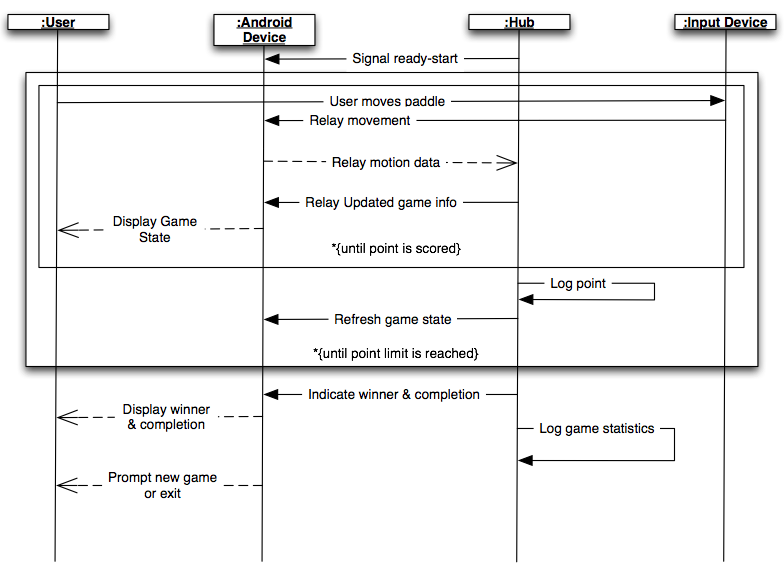
\includegraphics[scale=.5]{SystemSeq.png}
\caption{\label{System Sequence Diagram}The role of our system in gameplay is 
  described through the system sequence diagram above.}
\end{center}
\end{figure}


\subsubsection*{Initializing a Game - v3.0}
Actors:
\begin{itemize*}
\item Player
\item Hub
\item Device
\end{itemize*}
Preconditions:
\begin{itemize*}
\item The application is installed and open on the device.
\item The player has already created an account with Vir-Pong.
\item The input device is tethered to the Android device and is ready to 
  submit motion data.
\end{itemize*}
Postconditions:
\begin{itemize*}
\item The hub is relaying game information.
\item The system is using a display to relay the game state.
\end{itemize*}
Scenario:
\begin{enumerate*}
\item \label{InitGame_DisplayOptions} The software displays various options.
\item \label{SelectStart}The player selects to begin a game.
\item \label{DisplayGameRooms} The player is prompted with a list of various
game rooms.
\item \label{SelectRoom} Player selects the desired game.
\item \label{SystemRequestsGame}The device requests the selected game from 
the hub.
\item \label{NotifyPaddle} The player is notified of which paddle she is.
\item \label{HubSelectsOpponent}The hub waits for an opponent then signals a 
  ready-start to device.
\item \label{LoadGameState}The device loads an initial game state displayed 
  to the player.
\item Game begins.
\end{enumerate*}
Alternatives:\\
\ref{SelectStart}a) The player selects the wrong action.
\begin{enumerate*}
\item The player may elect to go back the the previous screen with a 
  $return$ function.
\end{enumerate*}

\ref{SystemRequestsGame}a) The system can not connect to the hub.
\begin{enumerate*}
\item The device sends the player an error message that prompts the player 
  to retry or exit.
\item Player chooses to retry.
\item System connects to hub.
\item Return to \ref{HubSelectsOpponent} of main scenario.
\end{enumerate*}

\subsubsection*{Connect to Input Device - v2.0}
Actors:
\begin{itemize*}
\item Player
\item Device 
\item Wii Remote
\end{itemize*}
Preconditions:
\begin{itemize*}
\item System is installed on the device and has launched.
\end{itemize*}
Postconditions:
\begin{itemize*}
\item Input device (Wii Remote) is selected and prepared for game use.
\end{itemize*}
Scenario:
\begin{enumerate*}
\item Player is prompted with options for input devices.
\item \label{SelectInput} Player selects to use a Wii Remote, but Wii Remote
is not connected yet.
\item \label{PromptToConnect} Device directs player to instructions for 
pairing with a Wii Remote.
\item \label{MenuToWii}Following directions, the player opens the correct 
menu for pairing with a Wii Remote.
\item Player selects to pair with the Wii Remote.
\item \label{ConnectWiimote}System attempts to tether Wii Remote.
\item Player follows instructions from system to connect Wii Remote.
\item System accepts Wii Remote device and notifies user.
\end{enumerate*}
Alternatives:\\
\ref{SelectInput}a) Player selects phone accelerometer.  
\begin{enumerate*}
\item System asks player to make certain the device has an built in 
  accelerometer.
\item Player indicates that device has accelerometer.
\item System connects to device accelerometer.
\item System proceeds to game launch.
\end{enumerate*}
\ref{SelectInput}b) Player selects touch screen interface.
\begin{enumerate*}
\item System asks player to touch a box displayed on-screen to ensure 
  that a touch screen is available.
\item Player touches box.
\item System proceeds to game launch.
\end{enumerate*}
\ref{ConnectWiimote}System attempts Wii Remote connection, and fails.
\begin{enumerate*}
\item System alerts user that connection failed.
\item User is prompted to try again or back out.
\end{enumerate*}

\subsubsection*{Changing the Game Settings - v2.0}
Actors:
\begin{itemize*}
\item Player
\item Device
\end{itemize*}
Preconditions:
\begin{itemize*}
\item The application is installed and open on the device.
\end{itemize*}
Postconditions:
\begin{itemize*}
\item The newly changed settings have been saved and will be applied to 
  future game play.
\end{itemize*}
Scenario:
\begin{enumerate*}
\item Main menu options are displayed to the player.
\item \label{SelectChangeSettings}Player selects a $change$ $settings$ 
  function.
\item \label{ChangeSettings}Player changes the setting(s).
\item \label{SelectSave}Player selects a $save$ $and$ $apply$ function.
\item \label{SystemSaves}Device saves changes and applies them to future 
  game plays.
\item \label{ReturnToMainMenu}Device returns to the main menu.
\end{enumerate*}
Alternatives:\\
\ref{ChangeSettings}a) The player selects a non-valid entry for a setting.
\begin{enumerate*}
\item The device displays an error message that tells the player he 
  entered a non-compatible value.
\item The device returns the setting to a default state.
\end{enumerate*}
\ref{SelectSave}a) The player decides not to change any settings.
\begin{enumerate*}
\item The player selects the $return$ function.
\end{enumerate*}
\onehalfspacing

\singlespacing
\subsubsection*{Viewing Replays - v2.0}
Actors:
\begin{itemize*}
\item Player
\item Website
\item Device
\end{itemize*}
Preconditions:
\begin{itemize*}
\item Our application is installed on the device and has launched.
\item The player has already created an account with Vir-Pong and is logged
  in.
\end{itemize*}
Postconditions:
\begin{itemize*}
\item The player has watched their replay.
\end{itemize*}
Scenario:
\begin{enumerate*}
\item Main menu options are displayed to the player.
\item \label{SelectReplay}Player chooses to view replay.
\item \label{ReplayChoice}Device requests list of available replays from server.
\item Database sends list of replays.
\item Device displays list of replays.
\item \label{WatchReplay}Player selects a replay to watch.
\item Device displays replay.
\item \label{Back}Player finishes the replay and hits the back button.
\item Device returns to main menu.
\end{enumerate*}
Alternatives:\\
\ref{PersonalStatRequest}a) Unable to obtain available replays.
\begin{enumerate*}
\item Display connection error message.
\item Player may utilize a $retry$ or $continue$ button.
\item Player selects $retry$.
\item Return to \ref{PersonalStatRequest}.
\end{enumerate*}

\subsubsection*{Editing Account Information - v1.0}
Actors:
\begin{itemize*}
\item Player
\item System
\item Vir-Pong Website
\end{itemize*}
Preconditions:
\begin{itemize*}
\item The application is installed on the device and has launched.
\end{itemize*}
Postconditions:
\begin{itemize*}
\item Player has edited account information.
\end{itemize*}
Scenario:
\begin{enumerate*}
\item Player selects Edit Account information on main menu.
\item Device displays current login and pin number.
\item Player may change these current settings.
\item Player saves and exits editing account information.
\item System returns user to previous page.
\end{enumerate*} 

\onehalfspacing



%    System Sequence Diagram:
%        Create a system sequence diagram for your most important 
%        fully-dressed use case. Include a one paragraph description of what 
%        is being depicted in the diagram (use plan English). 






\subsection{Nonfunctional Requirements}
%The product provides an extremely fun basic pong game that combines the use
%     of smart phones, Wii remotes, and server and web communication. It is 
%     free to use and open source available at https://github.com/VirPong/human-pong 
%     for developers. The developer documentation can be found on github or on the 
%     VirPong website. It will be launched on December 14th 2011 which is available 
%     to any person who wants to come see it at 4:00PM on the University of Puget 
%     Sound campus. It is accessible to people on the World Wide Web through our 
%     website and available to anyone who chooses to do so. A group will need two 
%     phones Android or iPhone, two Wiimotes, and be able to connect to our server 
%     in order to play. It works with most android phones except for those with 
%     SenseUI which has errors with the Bluetooth stack. See the VirPong website for 
%     the full user installation instructions and basic tutorial. A user has the 
%     choice of creating an account via the website or playing as a guest. Personal 
%     information saved in account is extremely secure. The product’s use of a pin 
%     number means your password is safe and doesn’t need to be encrypted or even 
%     known by the phones. Support can be found on the website but once everything 
%     needed to play the game is set up, a user can connect a Wii Remote to his phone, 
%     connect to the server and start a game against another player. The intuitive 
%     interface allows users to navigate and use the different functions of the 
%     product through the use of simple but distinct and easy to select buttons. 
%     Users can change certain settings for the game which will be saved over multiple 
%     uses.  Once in a game, activating the Wii Remote sends changes in the paddle 
%     position to the phone which then sends it to the server. The server receives 
%     these changes and sends an updated game state to the phones every 50 ms. If 
%     connection to  game fails, the program will promptly pause the game and notify you of the disconnection, however unfortunately you cannot resume the game from its state at disconnection.


\section{Diagrammatic Depictions of the Product}
\label{sec:diagrams}
%Domain Analysis: Create a UML diagram that depicts the domain model for your
%    product (this will be a revision from Report 1). Include a plain-English
%    description of what is being shown in the diagram. Define any terms used
%    in conceptual classes, attributes, or associations that might not be 
%    clear to a lay person.
<<<<<<< HEAD
\textbf{Figure~\ref{domainModel}} shows the interactions that take place and the associations involved in playing a game of virtual pong on an android device.  Throughout the game, the user controls an input device that will pass motion data to the android device.  There are three different types of input that can be used by the user: the Wii Remote, the phone accelerometer, or the touch screen interface.  The motion data from the input device is sent to the android device and immediately sent to the hub.  The hub sends back information on both the user's and an opponent's positions as well as the position of the ball.  Other relevant data is sent to and from the android device and hub, including score data and a signal that a point has been scored.  To allow the user to view their virtual pong game, the android device relies on a game interface to graphically display the constantly updating state of the game.  This game interface contains a graphical representation of two paddles and one ball that respond to information sent from the hub.
=======
\textbf{Figure~\ref{domainModel}} shows the interactions that take place and the associations involved in playing a game of Pong on an android device.  Throughout the game, the player controls an input device that will pass motion data to the android device.  There are three different types of input that can be used by the user: the Wii Remote, the phone accelerometer, or the touch screen interface.  The motion data from the input device is sent to the android device and from there is immediately sent to the hub.  The hub sends back information on both the player's and an opponent's positions as well as the position of the ball.  Other relevant data is sent to and from the android device and hub, including score data and a signal that a point has been scored.  To allow the player to view their Pong game, the android device relies on a game interface to graphically display the constantly updating state of the game.  This game interface contains a graphical representation of two paddles and one ball that respond to information sent from the hub and also keeps track of the game's current score.
>>>>>>> upstream/master
\begin{figure}
\begin{center}
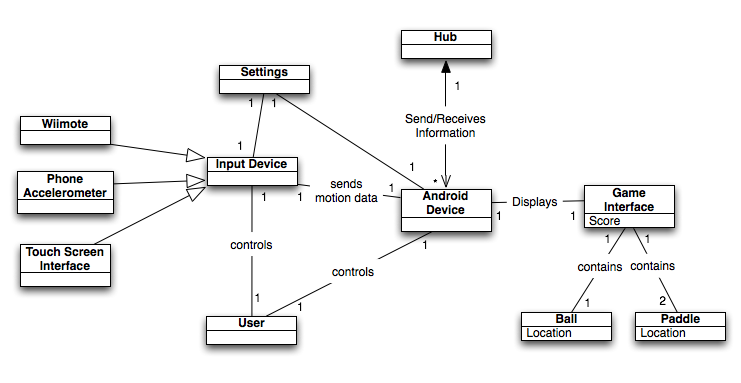
\includegraphics[scale=.7]{DomainModel.png}
\caption{\label{Domain Model} Class interactions and attributes outline the major system components.}
\end{center}
\end{figure}



%Interaction Diagram:
%    Create an interaction diagram for each of the events depicted in your 
%    System Sequence Diagram.
%    Add a description of the design principles (Information Expert, Creator,
%    High Cohesion, Low Coupling, Controller) you employed, where you employed
%    them and why you made those choices. 

\subsection{Interaction Diagram}
\begin{figure}
\begin{center}
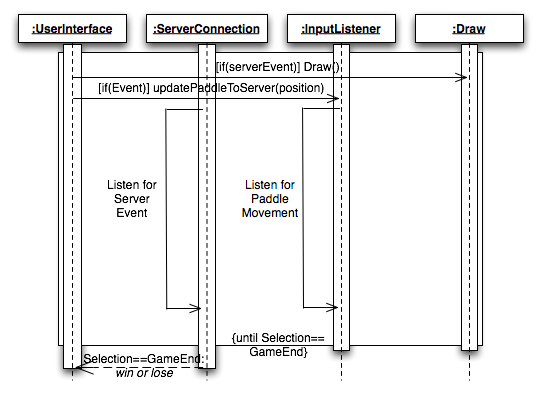
\includegraphics[scale=.7]{InteractionDiagram.png}
\caption{\label{InteractionDiagram}}
\end{center}
\end{figure}
Though our code utilizes a number of design patterns, the code for our first use case, playing a pong
game, uses three highly advantageous design patterns that help structure our code.
One of the design patterns used was the observer pattern.  In order to update paddle positions for each
player efficiently, we chose to listen for events from the input device rather than constantly updating
over specific increments of time.  We also utilized the information expert pattern in regards to drawing
and redrawing the screen during game play.  The server maintains the current game state, so the
serverConnection class has knowledge of the paddle and ball locations.  Consequently, the serverConnection
class is given the responsibility of calling the draw method so that the screen will represent the
current game state.  We also maintain high cohesion in our Draw class.  Draw is only focused on methods
involving the act of drawing a figure on to the canvas.  This makes the class highly cohesive and as a
result, the code is easily understood and can be reused.

\section{Implementation}
\label{sec:implementation}
%Implementation:
%    Include the coding style guide that your team is using. This should be 
%    fairly detailed including naming, coding conventions, and comment 
%    conventions.
%    Install documentation: include a description of all necessary procedures 
%    a developer would have to complete to install your product. If you are 
%    assuming a certain starting environment then explicitly state so (e.g. a 
%    Linux server with Apache installed). Make sure to include how the user 
%    would access and download your source code and documentation. If you had 
%    difficulty installing from the previous teams description be sure to 
%    correct those difficulties.
%    Include a current class diagram of your product
%        Diagram should depict all classes and their associations 
%    Description of algorithms, data structures and design patterns
%        Describe any complex algorithms, data structures, or design patterns 
%        your group used. Provide insights as to why you made the choices you 
%        did.
%        Describe any techniques you are using to ensure fault tolerance (e.g.
%        if you have information to write to a db but the db is down what do 
%        you do?) 
%    Data Storage:
%        Identify all the data you are storing (ex. user athentication, 
%        medical records, back up information if the DB is down etc.)
%        If your product contains a database include both an ER Diagram and 
%        the schema for it, include a description of why you made the design 
%        decisions you did.
%        If the data is not stored in a db describe how it is stored included 
%        formatting. 
%    Describe your testing and verification procedure for your implemented 
%    code 
%         

\section{Coding Style Guide}

The majority of the coding takes place within the $assets/www$ folder of our application.  It is, therefore, important that our team maintain a clear and concise style within this limited space.  In general, folders should be titled in the CamelCase style (first letter a capital) and individual files should be likewise with the exception that the first letter is a lower case.  Dashes may be permitted so long as it is used when there may be multiple editions of something (e.g. a "logo-blue.jpg" and "logo-red.jpg").  Further exceptions include any README files (used for build instructions) or versioned files. 



As to how many folders to have, if there exists a logical grouping between one file and several others (i.e. more than 2 files are related to one another) then these should be placed in a separate folder within the $www$ directory.  Files themselves and the code contained should follow the guidelines given below.  While these guidelines are not quite as extensive as some resources (such as Sun's own Java style guide\cite{JavaStyle-Sun}) the brevity serves our team well.



\subsection{Working with Java}

While Java is not a primary language for our team, we will be strictly following conventions laid down by Sun and other programmers\cite{JavaStyle-Sun}\cite{JavaStyle-JavaRanch}.



\subsubsection{Style Rules}

\begin{itemize}

\item All identifiers use letters ('A' through 'Z' and 'a' through 'z') and numbers ('0' through '9') only. No underscores, dollar signs or non-ascii characters (with one exception mentioned later).

\item In general, use $methodNamesLikeThis$, $variableNamesLikeThis$, $ClassNamesLikeThis$, and $SYMBOLIC\_CONSTANTS\_LIKE\_THIS$.

\item Use a separate line for an increment or decrement.

\item All fields must be private, except for some constants.

\item Class elements will follow this order: fields, constructors, methods.

\item Limit the scope of local variables.

\item Initialize objects as late as possible.

\item Use Strings with care.

\item Avoid wrapper classes.

\end{itemize}

\textbf{A note on comments:} all methods and classes should contain a standard Javadoc comment (text description and appropriate author, version, parameter and return tags).  In-line comments are strongly encouraged to assist in readability of the code.



\subsubsection{Coding Rules}

\begin{itemize}

\item Opening curly braces should be on the same line as what they are opening.

\item Closing curly braces will be horizontally aligned with the line where the statement began.

\item Indent each time a new bracket set is created.  Indents should be four spaces.

\item All control-flow statements must use brackets.

\item Commas and semicolons are always followed by whitespace.

\item Binary operators should have a space on either side.

\item Parentheses should be used in expressions not only to specify order of precedence, but also to help simplify the expression. When in doubt, parenthesize.

\item There will be no use of $break$.

\end{itemize}





\subsection{Working with JavaScript}

The majority of our JavaScript style guidelines are mimicked from Google\cite{JavaScriptStyle-Google}.  For further and more detailed information, see their guide.  To many new programmers, JavaScript seems very much like Java (even the name!), but it is important to note that these are different languages and we have several very different rules.



\subsubsection{Style Rules}

\begin{itemize}

\item In general, use $functionNamesLikeThis$, $variableNamesLikeThis$, $ClassNamesLikeThis$, $EnumNamesLikeThis$, $methodNamesLikeThis$, and $SYMBOLIC\_CONSTANTS\_LIKE\_THIS$.

\item Avoid using many global variables.

\item Start curly braces on the same line as what they are opening.

\item Be sure to indent blocks by four spaces.

\item Use blank lines to group logically related pieces of code.

\item Use parentheses only when required.

\item Prefer $'$ over $"$ for strings.

\item Be sure to use JSDoc comments.  A comment at the top of the file for authorship and general overview, comments for methods, and inline comments are encouraged.  The first two are done using $/*. . . */$ and the latter is $//$.

\item Use JSDoc annotations ($@private$ and $@protected$) where appropriate.  Marking visibility is encouraged.

\item Be sure to use @param and @return tags for methods and functions.

\item Simple getters may have no description but should specify the returned values.

\end{itemize}



\subsubsection{Coding Rules}

\begin{itemize}

\item Always declare variables with $var$.

\item Use $NAMES\_LIKE\_THIS$ for constants. Use $@const$ where appropriate. Never use the $const$ keyword.

\item Always end lines with semicolons.

\item Feel free to use nested functions but try to comment these to make them clear.

\item Avoid wrapper objects for primitive types.

\item The keyword $this$ is for object constructors and methods only.

\item For-in loops are only for iterating over keys in an object/map/hash.

\item Do not use multiline string literals.  Instead, use concatenation when initializing such long strings.

\item Use $onclick$ instead of $javascript:$ for anchors.

\end{itemize}



\subsection{Working with HTML5}

HTML5 and CSS are so quickly evolving of late that style guides are not readily available.  We have, however, compiled our own unique guide from some suggestions found on the Web Developer's Virtual Library\cite{HTMLStyle-WDVL}.  We recommend keeping JavaScript and CSS code in files separate from the HTML.  This is primarily to keep the code modular and sensible.  Reading HTML and JavaScript in the same file can be confusing.



\begin{itemize}

\item Block-level tags are to the far left with content indented four spaces.

\item Don't indent tags relative to their container.

\item Line up multiple attributes with the "=" signs all in the same column.

\item The home page is an index to other pages.

\item Page designs should be consistent in appearance and structure.

\item Choose a meaningful title for pages.

\item $*$Unless it is an incredibly brief code-snippet, do not include JavaScript or CSS in the $html$ file.  Place this code in a separate file.

\item Provide a $Home$ link.

\end{itemize}



\subsection{Style Guide Removal}

Due to the fact that we have redistributed tasks among the two phone teams, we have removed some items that no longer apply to the Android Development team.  The following have been removed: 



\begin{itemize}

\item CSS style guide section

\end{itemize}

\section{User Documentation}
\subsection{Features Overview}
 VirPong provides a safe and fun pong game that combines the use of connections and communication between Wii Remotes, smart phones, and a local University of Puget Sound Server. This allows you to play pong against another human player using your phone and a Wii Remote as a controller.

\subsection{Setting Up}
Setting up VirPong game environment and account is simple and quick. It allows for the convenient set up of everything entirely from your phone through the use of our website.
\begin{itemize}
\item The product can be downloaded by directing your Android internet browser to “WEBSITE” and clicking on the Android APK download. An automatic prompt asking if you want to install the APK should pop up. Follow your phones instructions to complete installation of the application.
\item Follow the instructions on the website to quickly and easily set up your own VirPong user account, information, and password. If you do not want to do this, you also have the choice of not logging in and using a guest account.
\item Once your user account has been set up launch the application.
\end{itemize}
\subsection{Functions of the Main Menu}
\begin{figure}
\begin{center}
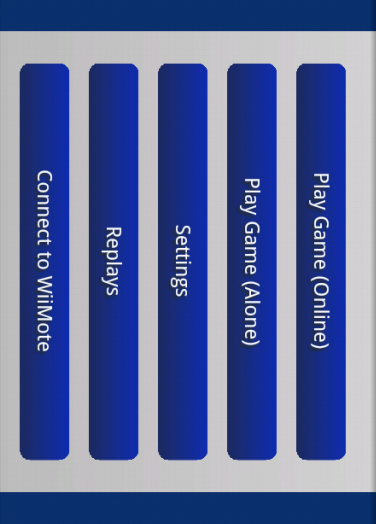
\includegraphics[scale=.7]{homeScreen.png}
\caption{\label{homeScreen}Home Screen Menu}
\end{center}
\end{figure}

\subsubsection{User Settings}
\begin{figure}
\begin{center}
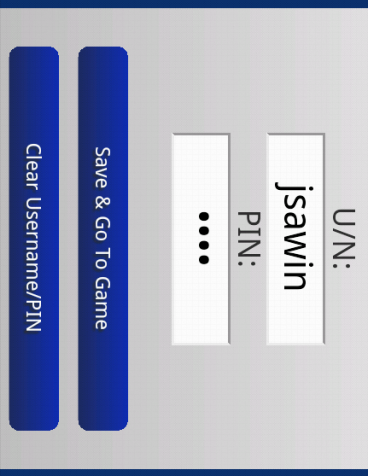
\includegraphics[scale=.7]{userNamePinSave.png}
\caption{\label{User Setting Interface}User Settings Menu}
\end{center}
\end{figure}

The first thing a user will probably want to do upon opening the application for the first time is opening the settings page. This will bring up a page that allows the user to put in their username and pin number that will save so they can stay logged in through multiple uses.
\subsubsection{Select Input Method}
\begin{figure}
\begin{center}
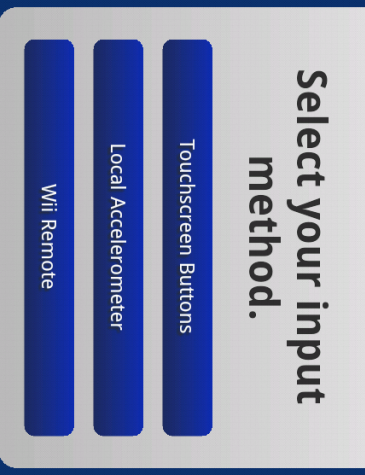
\includegraphics[scale=.7]{selectInputMethod-Android.png}
\caption{\label{Input Selection Interface}Input Selection Menu}
\end{center}
\end{figure}

After saving any settings, the user will want to select the input method and follow the correct steps to set up the input device.
\begin{itemize}
\item Wii Remote – choose this under input options and run the plugin in order to use a Wii Remote as your controller. The plugin should pop up and allow you to connect to the Wii Remote. Once connection has been verified you are ready to play a game.
\item Phone Accelerometer – this option will allow you to use the phones accelerometer rather than the Wii Remote. This allows you to play if you don’t have a Wii Remote.
\item Button Presses – choosing this input method will allow you to play the game by using button presses on the screen to move your paddle.
\end{itemize}
\subsubsection{Play Game}
Upon selecting the Play Game on Internet option, the application will bring you to a page containing different game rooms. 
\begin{figure}
\begin{center}
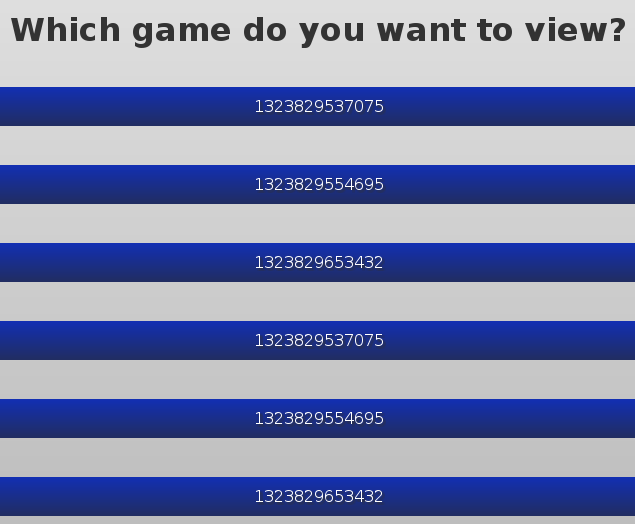
\includegraphics[scale=.7]{gameSelect.png}
\caption{\label{gameSelection}List of Joinable Games Menu}
\end{center}
\end{figure}

\begin{itemize}
\item Choosing a game with one person already in it will allow you to join the game and start playing versus them.
\item You can choose to create a new game, where you will have to wait until another player joins to start.
\item Or you can join a game that already has two players and watch them play as an observer.
\end{itemize}
You can also choose to play offline against a simple bot program in order to test your skills when an opponent is no longer available.
\begin{figure}
\begin{center}
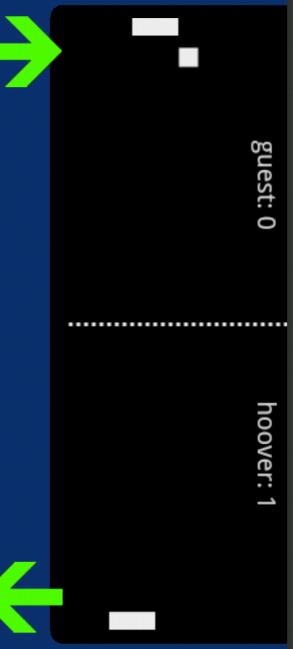
\includegraphics[scale=.7]{ touchOnServer.png}
\caption{\label{PlayingGame}Game in Action}
\end{center}
\end{figure}

\subsubsection{Replay Game}
After you have played a game or even if you haven’t and just want to watch a replay of a game, select the function to watch a replay. This will bring up a selection of previously played games to watch from.
\subsection{Rules of Pong}
Now for the fun, playing pong is extremely simple and fun. The rules are straight forward and any new player can pick them up easily. Here are the basics:
\subsubsection {Major Components}
There are 3 major components to any pong game. These are the ball, the paddles, and score area. 
\begin{itemize}
\item Ball – flies around the screen following basic game mechanics and doing basic collision detection. If this makes it into your score area, you lose a point.
\item Score area – this is everything between your paddle and the end of the screen. 
\item Paddle – this is the only thing the user controls. The game will tell you which of the two is yours and use of your selected input method will cause it to move up and down on the screen. 
\subsubsection{How to Play}
The basic concept of a pong game is to hit the ball with your paddle more than your opponent does. Try to send the ball flying into your opponents score area while still defending your score area from balls your opponent sends flying at you. The first to 10 points wins.




\section{Developer Documentation}

\label{sec:developerdocumentation}

\subsection{Setting up the Development Environment}
In order to develop for Android, you will need the Android SDK, the PhoneGap software, and some editor (for example, Eclipse).  These pieces are relatively easy to set up, but because all systems are different, some personal configuration may be required.  All of the software mentioned below can be found, with current links, at the PhoneGap Android page\cite{PhoneGap-Android}.  

\subsubsection{Android SDK}
The Android SDK comes with an Android Emulator as well as Android libraries.
To download the SDK, first check to make sure your operating system fulfills all of the system requirements.  A list of of system requirements is available on the Android Developers website\cite{AndroidSDK-SystemRequirements}.

Next, download the Android SDK from the Android Developer website\cite{AndroidSDK-Download}.
The instructions for installation are found on the same site but on the installation page\cite{AndroidSDK-Installation}. \textbf{Note:} do not put a space in the folder name.

After that, you must add necessary components to the SDK.  The instructions for that portion are found on the components page\cite{AndroidSDK-Components}.  On your first run, you will be required to create an Android Virtual Device (AVD) that is simply a mock phone.


\subsubsection{PhoneGap}
The PhoneGap download is primarily a collection of tools that provide functionality for the HTML5 and JavaScript interface in a native application environment.  That is, the PhoneGap jar, js, and xml files all serve to support the use of HTML5 and JavaScript coding as implementing the core functionality of the application.  The download for PhoneGap can be found on the PhoneGap Android page\cite{PhoneGap-Android}.


\subsubsection{Editing Environment}
In theory, any development can be done from a text editor so long as you have access to the Android SDK and Java.  It is highly recommended, however, that you use Eclipse\cite{Eclipse-Helios}.  You then may want to install the ADT plugin for Android Development\cite{Eclipse-ADT}.  In addition, you may then want to install the plugin for PhoneGap Development\cite{PhoneGap-Eclipse}.

\textbf{An important note:} When creating a PhoneGap application in Eclipse, it may be necessary to include the PhoneGap jar file in the libs folder of the application.  To do this, right-click on the Eclipse project, and select "Build Path", then "Configure Build Path".  If there is no PhoneGap jar file included, then select to "Add External JARs".  Select the jar file downloaded earlier with the rest of the PhoneGap tools and click "Okay".

\subsection{Retrieving the Source}
<<<<<<< HEAD
In order to work with the source code of the project, you will likely want to use Git\cite{Github}.  Using Git, you may clone the repository from \url{git@github.com:VirPong/human-pong}.  You will then want to navigate into $Android/VirPong-Mobile/$ and create a folder called $assets$.  Navigate into $assets$ and clone \url{git@github.com:VirPong/www}.  Now you may open Eclipse and import the $VirPong-Mobile$ directory as an existing project.  You may need to point the build path to your PhoneGap Jar file (located wherever you downloaded PhoneGap and then inside the Android folder).  Once this is done, you may begin development!  \textbf{Note:} an alternative to git is to download the repository from \url{https://github.com/VirPong/human-pong} and \url{https://github.com/VirPong/www}, placing the $www$ repository in the same place mentioned above.
=======
In order to work with the source code of the project, you will likely want to use Git\cite{Github}.  Using Git, you may clone the repository from \url{git@github.com:Vir-Pong/human-pong}.  You will then want to navigate into $Android/Vir-Pong-Mobile/$ and create a folder called $assets$.  Navigate into $assets$ and clone \url{git@github.com:Vir-Pong/www}.  Now you may open Eclipse and import the $Vir-Pong-Mobile$ directory as an existing project.  You may need to point the build path to your PhoneGap Jar file (located wherever you downloaded PhoneGap and then inside the Android folder).  Once this is done, you may begin development!  \textbf{Note:} an alternative to git is to download the repository from \url{https://github.com/Vir-Pong/human-pong} and \url{https://github.com/Vir-Pong/www}, placing the $www$ repository in the same place mentioned above.
>>>>>>> upstream/master

\section{Class Diagram}
\begin{figure}
\begin{center}
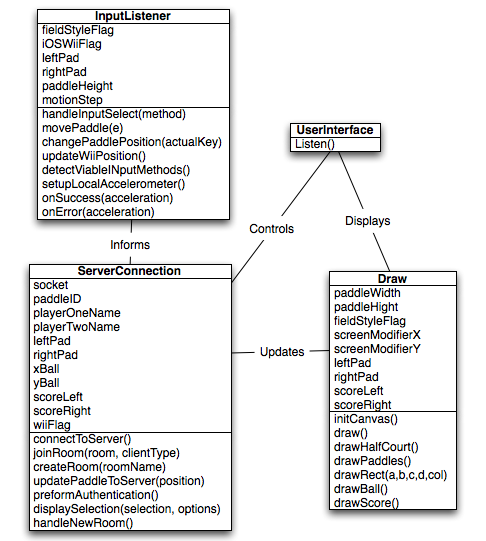
\includegraphics[scale=.5]{ClassDiagram.png}
\caption{\label{Class Diagram}This model depicts the all the classes and their associations within our pong.js file.  The ServerConnection class updates the Draw class, and continually calls to redraw the canvas.  The ServerConnection also is informed by InputListener as to what input is being used and when it updates position.  The UserInterface displays the refreshed canvas from Draw, and is controlled by ServerConnection as far as the game state.}
\end{center}
\end{figure}

\section{Database}
In order to enforce security of the highest, the smart phones do not deal with the user password which is the only thing that allows access to personal information stored with the account. Instead the phones only store the user name and a pin number that grants the user limited access. This means that all major account settings and changes can only happen through the website. The account information saved on the phone uses HTML5 localstorage and more information and tutorials on localstorage can be found at http://www.w3schools.com/html5/html5_webstorage.asp. It uses JavaScript to store and access data and provides a more efficient replacement for cookies in webpages. It provides easy saving and accessing using a lookup key for each pin number and account name.

\section{Reflections}
\label{sec:reflections}
%Reflections:
%    Describe the technical challenges you encountered in the development of 
%    your product.
%    Describe how the software engineering techniques you learned in this 
%    course helped you in your development.
%    Describe what you would have done differently if you were to start this 
%    project over again.
%    If you were to continue this project what would you do. 
<<<<<<< HEAD
The biggest challenge involved with a project of this nature is the variety of interactions between all of the groups.  The Android device in particular relies on communication with the Wii Remote, server, and website, so consistent communication is vital.  Therefore, if one team manager does not make an effort to communicate, the entire project suffers.  We finally realized the importance of human communication and have had more manager meetings than at the beginning of the semester.  In addition, managers have become more prompt with emailing and this has made it much easier to stay in touch and keep everyone updated on the status of the project.  Another challenge has been a general lack of motivation due to a failure to create a sense of individual accountability.  It was nearly impossible to measure how much work each individual in every group had done; consequently, team members were not highly motivated to work at a fast pace.  As a result, some teams would move ahead of the others and then feel a great deal of frustration when they had to wait for other teams to catch up.  This is an extremely difficult challenge to overcome, but the situation has improved because we have reached the point where it is apparent if a team member is not contributing a satisfactory amount.  The increased manager communication also causes the group leaders to hold each other more accountable for their group’s progress.  A more specific challenge for the Android team was getting the iOS development team to agree to implement PhoneGap; this was difficult because their team members were divided on the issue.  This was especially frustrating because our team couldn’t move forward until the iOS team had made their decision.  However, we finally convinced them that the use of PhoneGap has a number of important benefits.

If we were to begin this project again, there are a number of things we would have done differently.  First of all, we would have written the APIs for Android to server and Android to Wii Remote communication at the very start of the project.  This would have allowed our team to more forward, even when the other teams were stuck.  This change would also have helped us be clearer in our expectations of what we needed from the Wii Remote team.  Another beneficial change would been restructuring the Android and iOS development teams.  Since we are using PhoneGap, the user interface for the game will be the same for both systems, so it would have been advantageous to instead divide the teams between “local” programming (the interface, pong game, features) and communications (namely between the server and the device, but also the Wii Remote to the device). 
=======
The biggest challenge involved with a project of this nature is the variety of interactions between all of the groups.  The Android device in particular relies on communication with the Wii Remote, server, and website, so consistent communication is vital.  Therefore, if one team manager does not make an effort to communicate, the entire project suffers.  We finally realized the importance of human communication and have planned more manager meetings for the rest of the semester.  In addition, managers have become more prompt with emailing and this has made it much easier to stay in touch and keep everyone updated on the status of the project.  Another challenge has been a general lack of motivation due to a failure to create a sense of individual accountability.  It was nearly impossible to measure how much work each individual in every group had done; consequently, team members were not highly motivated to work at a fast pace.  As a result, some teams would move ahead of the others and then feel a great deal of frustration when they had to wait for other teams to catch up.  This is an extremely difficult challenge to overcome, but the situation has improved because we are at the point where it is apparent if a team member is not contributing a satisfactory amount.  The increased manager communication also causes the group leaders to hold each other more accountable for their group’s progress.  A more specific challenge for the Android team was getting the iOS development team to agree to implement PhoneGap; this was difficult because their team members were divided on the issue.  This was especially frustrating because our team could not move forward until the iOS team had made their decision.  However, we finally convinced them that the use of PhoneGap has a number of important benefits for both teams.

If we were to begin this project again, there are a number of things we would have done differently.  First of all, we would have written the APIs for Android to server and Android to Wii Remote communication at the very start of the project.  This would have allowed our team to more forward, even when the other teams were stuck.  This change would also have helped us be clearer in our expectations of what we needed from the Wii Remote team.  Another beneficial change would been restructuring the Android and iOS development teams.  Since we are using PhoneGap, the user interface for the game will be the same for both systems, so it would have been advantageous to instead divide the teams between “local” programming (the interface, pong game, features) and communications (namely between the server and the device, but also the Wii Remote to the device). 
>>>>>>> upstream/master



%%%%%%%%%%%%%%%%%%%%%%%%%%%%%%%%%%%%%%%%%%%%%%%%%%%%%%%%%%%%%%%
%8. References: Clearly indicate all the tools and sources you have used in the development of your product thus far. 
%%%%%%%%%%%%%%%%%%%%%%%%%%%%%%%%%%%%%%%%%%%%%%%%%%%%%%%%%%%%%%%


\newpage
\bibliographystyle{amsplain}
\bibliography{finalReport.android.bib}








\end{document}